
\documentclass[a4paper,12pt]{article}

\usepackage[utf8]{inputenc}
\usepackage[T1]{fontenc}
\usepackage{graphicx}
\usepackage{float}
\usepackage{geometry}
\usepackage{booktabs}
\usepackage{tikz}

\usetikzlibrary{arrows.meta,positioning}

\geometry{margin=2.5cm}

\setlength{\parindent}{0pt}
\setlength{\parskip}{0.5em}

\title{Bericht}
\author{Jiaqi Wang}
\date{\today}

\begin{document}

\maketitle


\section{Hardware-Verbindungsdiagramm}

Mit der Software Fritzing wurde ein Schaltplan für die Hardwareverbindungen erstellt. Dadurch sind die elektrischen Verbindungen übersichtlich und klar erkennbar. Außerdem dient der Schaltplan als Grundlage für die spätere Verdrahtung und das anschließende Löten der Schaltung.

Das erstellte Hardware-Verbindungsdiagramm ist in Abbildung~\ref{fig:hardware_connection} dargestellt.

\begin{figure}[H]
    \centering
    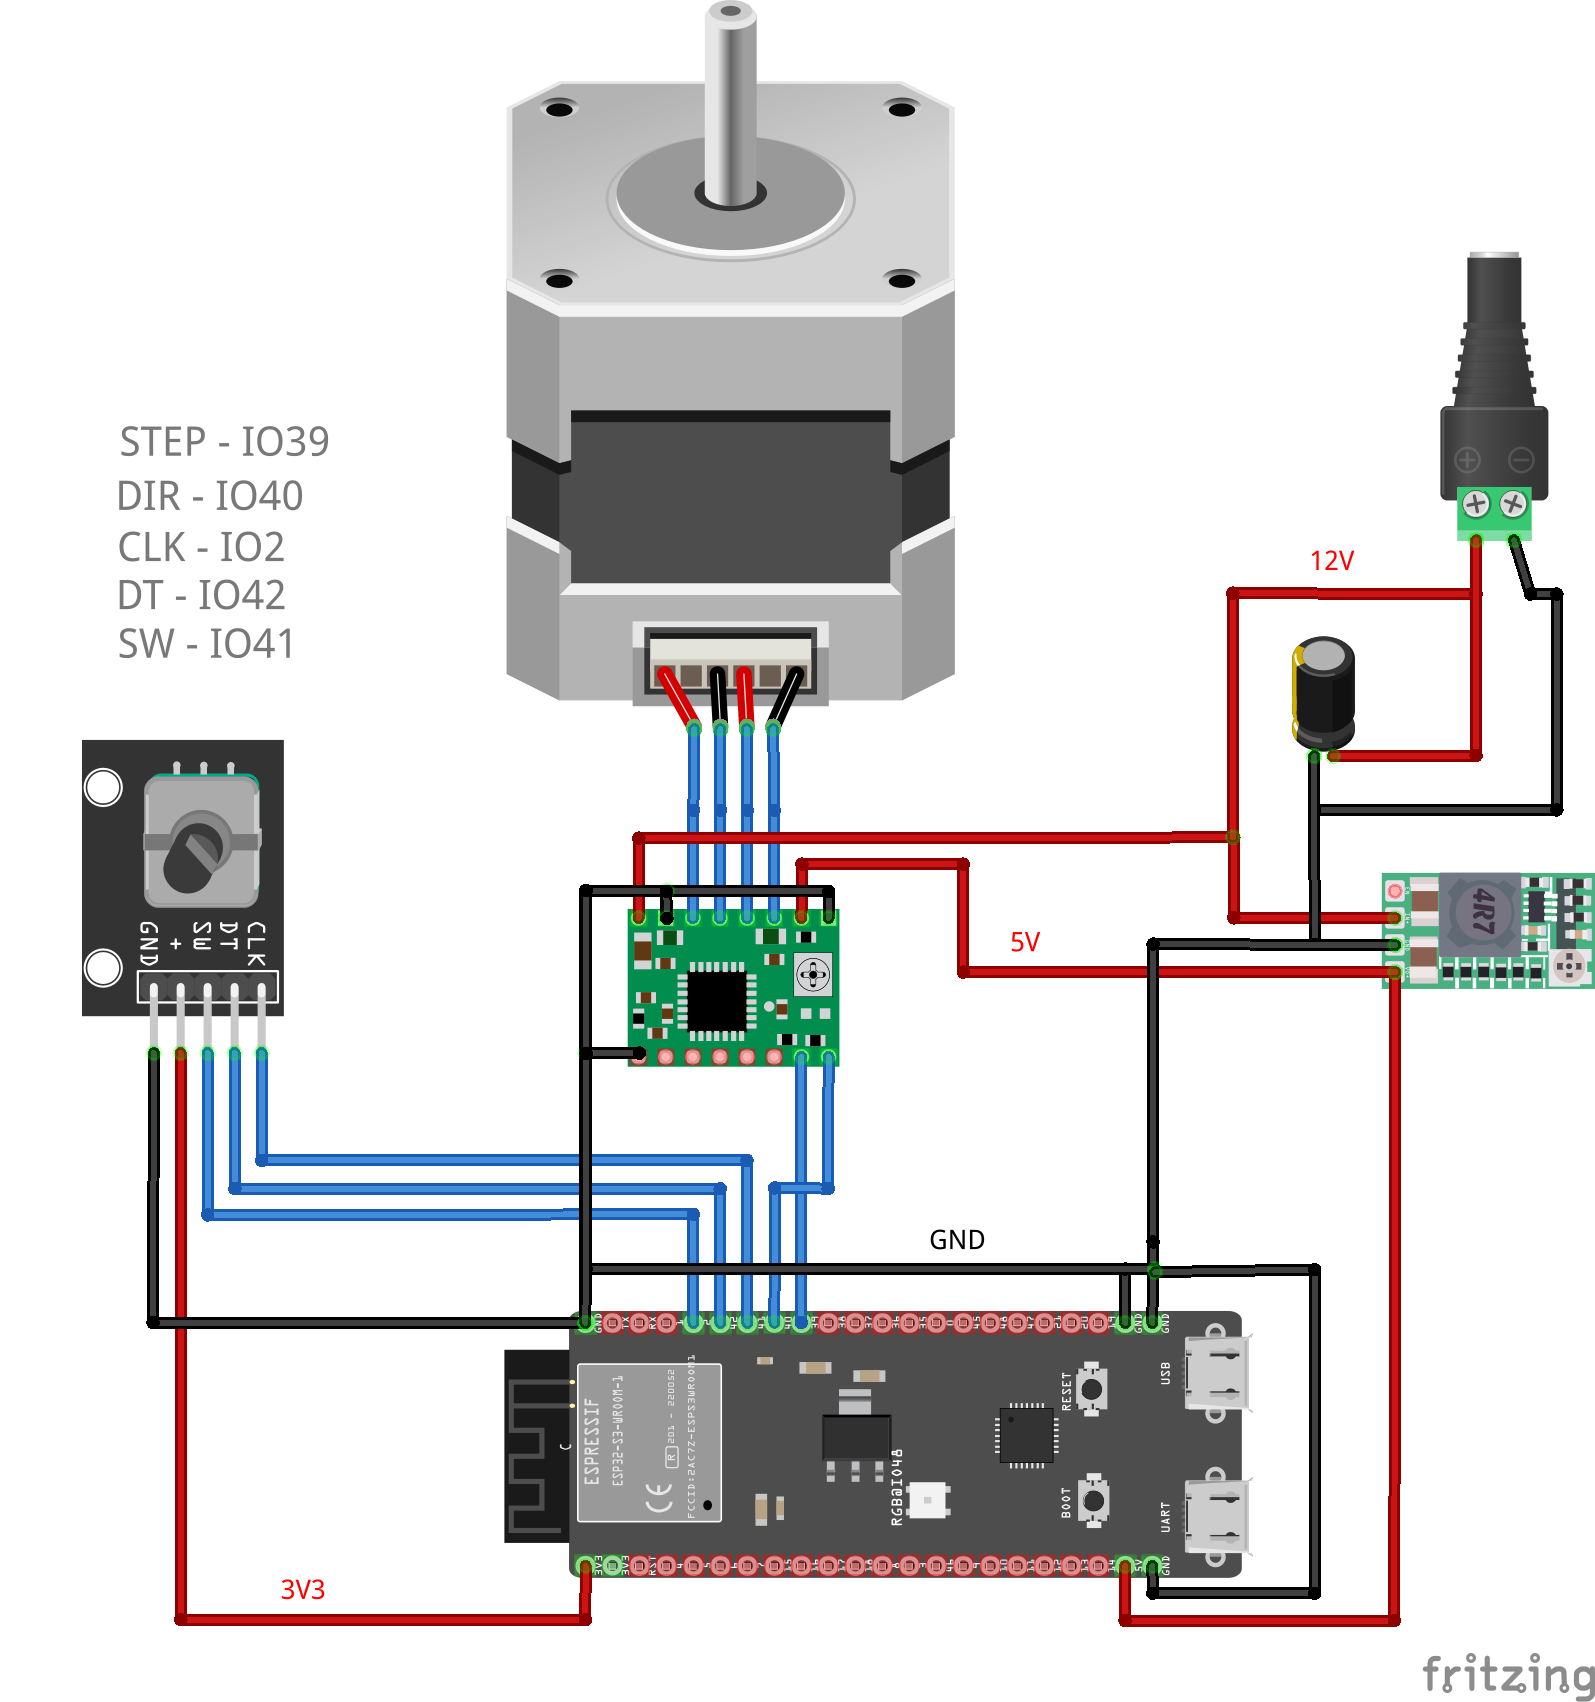
\includegraphics[width=0.6\textwidth]{hardware_connection.png}
    \caption{Hardware-Verbindungsdiagramm des Versuchsaufbaus}
    \label{fig:hardware_connection}
\end{figure}




\section{TCP-Kommunikation und Closed-Loop-Steuerung}

In der verbesserten Version wurde die TCP-Kommunikation mit der Closed-Loop-Steuerung kombiniert. Dadurch kann der Schrittmotor über WLAN ferngesteuert werden. Die vom PC gesendeten Winkelbefehle werden vom ESP32-S3 empfangen und anschließend an die Motorsteuerung weitergegeben.

Da nicht an jedem Einsatzort ein 2{,}4\,GHz-WLAN verfügbar ist, wurde zusätzlich ein AP-Modus implementiert. Der ESP32-S3 kann somit entweder mit einem vorhandenen WLAN verbunden werden oder selbst einen WLAN-Hotspot bereitstellen. Der Wechsel zwischen beiden Modi erfolgt durch eine einfache \texttt{\#define}-Anweisung.

Das folgende Programmfragment zeigt die grundlegende Umschaltung zwischen WLAN- und AP-Modus:

\begin{verbatim}
#define NETMODE 1

WiFiServer server(8080);

void setupNetwork() {
#if NETMODE == 0
  WiFi.mode(WIFI_STA);
  WiFi.begin(WIFI_SSID, WIFI_PASS);

#elif NETMODE == 1
  WiFi.mode(WIFI_AP);
  WiFi.softAP(AP_SSID, AP_PASS);
#endif

  server.begin();
}
\end{verbatim}




\section{PID-Regelung zur Verbesserung der Genauigkeit}

Zur weiteren Verbesserung der Positioniergenauigkeit wurde die Closed-Loop-Steuerung um eine PID-Regelung erweitert. Dabei wird der Sollwinkel mit dem vom Drehgeber gemessenen Istwinkel verglichen. Aus der Differenz entsteht der Regelungsfehler, der vom PID-Regler verarbeitet wird. Das Ergebnis wird anschließend zur Anpassung der Schrittfrequenz des Motors verwendet.

\begin{figure}[H]
\centering

\begin{tikzpicture}[>=Stealth, node distance=1.6cm]

% Nodes
\node[circle, draw, minimum size=8mm] (sum) at (0,0) {$+$};
\node[draw, minimum width=2.5cm, minimum height=1.2cm, right=of sum] (pid) {PID-Regler};
\node[draw, minimum width=3.0cm, minimum height=1.2cm, right=of pid] (plant) {Motor + Treiber};
\node[draw, minimum width=2.5cm, minimum height=1.0cm, below=1.5cm of plant] (enc) {Drehgeber};

% Forward path
\draw[->] (-2,0) -- (sum) node[midway, above] {$x$};
\draw[->] (sum) -- (pid) node[midway, above] {$e$};
\draw[->] (pid) -- (plant) node[midway, above] {$u$};
\draw[->] (plant.east) -- +(2,0) node[midway, above] {$y$};

% Feedback
\draw[->] (plant.south) -- (enc.north);
\draw[->] (enc.west) -| (sum.south);

% Minus sign
\node at (-0.35,-0.55) {$-$};

\end{tikzpicture}

\caption{Blockdiagramm der Closed-Loop-Steuerung mit PID-Regler}
\label{fig:pid_closed_loop}
\end{figure}

In Abbildung~\ref{fig:pid_closed_loop} beschreibt \(x\) den Sollwinkel und \(y\) den gemessenen Istwinkel des Motors. Der Fehler \(e\) ergibt sich aus der Differenz zwischen Soll- und Istwert. Der PID-Regler berechnet daraus das Steuersignal \(u\), mit dem die Schrittfrequenz des Schrittmotors angepasst wird.

Der PID-Regler besteht aus drei Anteilen. Der P-Anteil reagiert direkt auf den aktuellen Fehler. Der I-Anteil berücksichtigt die aufsummierte Abweichung über die Zeit und kann bleibende Fehler reduzieren. Der D-Anteil reagiert auf die Änderungsgeschwindigkeit des Fehlers und kann Überschwingen verringern.

Das folgende Programmfragment zeigt den zentralen Teil der PID-Berechnung:

\begin{verbatim}
float error = targetAngle - currentAngle;

integral += error * dt;
float derivative = (error - lastError) / dt;

float pidOutput = pidKp * error
                + pidKi * integral
                + pidKd * derivative;

bool dir = error > 0.0f;
float usedSpeedHz = fabs(pidOutput);

if (usedSpeedHz < localMinSpeedHz) {
  usedSpeedHz = localMinSpeedHz;
}

if (usedSpeedHz > maxSpeedHz) {
  usedSpeedHz = maxSpeedHz;
}
\end{verbatim}

In diesem Programm wird der PID-Ausgang nicht direkt als Winkel verwendet, sondern zur Bestimmung der Schrittfrequenz. Die Drehrichtung wird durch das Vorzeichen des Fehlers bestimmt. Dadurch dreht der Motor in Richtung des Zielwinkels, während die Geschwindigkeit abhängig von der Größe des Fehlers angepasst wird.

Die verwendeten Standardparameter sind:


\begin{table}[H]
\centering
\caption{Einfluss der einstellbaren Regelungsparameter}
\renewcommand{\arraystretch}{1.25}
\begin{tabular}{p{2.6cm}p{2.2cm}p{4.6cm}p{4.6cm}}
\toprule
Parameter & Wert & Bei Erhöhung & Bei Verringerung \\
\midrule

\(K_p\)
& 5.0
& Der Motor reagiert schneller auf Positionsfehler. Bei zu hohem Wert kann es jedoch zu Überschwingen kommen.
& Die Reaktion wird langsamer. Die Zielposition wird weniger schnell erreicht. \\

\(K_i\)
& 0.015
& Bleibende Abweichungen werden stärker ausgeglichen. Ein zu hoher Wert kann jedoch zu Instabilität führen.
& Das System läuft ruhiger, aber ein dauerhafter Restfehler kann bestehen bleiben. \\

\(K_d\)
& 0.0
& Schnelle Fehleränderungen werden stärker gedämpft. Dadurch kann Überschwingen reduziert werden.
& Die Dämpfung wird geringer. Der Motor kann stärker nachschwingen. \\

Speed
& 500\,step/s
& Die Schrittfrequenz wird höher. Der Motor bewegt sich schneller, kann bei zu hoher Geschwindigkeit jedoch Schritte verlieren.
& Die Bewegung wird langsamer, dafür läuft der Motor meist stabiler. \\

Encoder CPR
& 40
& Eine höhere Impulszahl pro Umdrehung führt zu einer feineren Winkelauflösung, wenn der Encoder dies unterstützt.
& Eine niedrigere Impulszahl verringert die Winkelauflösung und kann die Positionsbestimmung ungenauer machen. \\

Tolerance
& 4.5°
& Die Zielposition wird früher als erreicht akzeptiert. Dadurch stoppt der Motor schneller, aber mit geringerer Genauigkeit.
& Die Positionsgenauigkeit steigt, jedoch kann der Motor länger nachregeln oder unruhiger werden. \\

\bottomrule
\end{tabular}
\end{table}



Zusätzlich können die Parameter Encoder CPR und Tolerance eingestellt werden. 
Encoder CPR beschreibt die Anzahl der Encoder-Impulse pro vollständiger Umdrehung. 
Aus diesem Wert berechnet der ESP32-S3 die Winkelauflösung des Drehgebers:

\[
\text{Winkel pro Impuls} = \frac{360^\circ}{\text{Encoder CPR}}
\]

Bei einem Wert von \(40\) entspricht ein Encoder-Impuls somit:

\[
\frac{360^\circ}{40} = 9^\circ
\]

Dieser Parameter muss zum verwendeten Drehgeber passen. Wenn der Wert falsch eingestellt ist, berechnet der Mikrocontroller eine falsche Winkelposition.

Der Parameter Tolerance gibt die zulässige Abweichung zwischen Sollwinkel und Istwinkel an. 
In der aktuellen Einstellung beträgt die Toleranz \(4.5^\circ\). 
Das bedeutet, dass die Bewegung als abgeschlossen gilt, sobald der Fehler kleiner oder gleich \(4.5^\circ\) ist.

Eine größere Toleranz führt dazu, dass der Motor schneller stoppt, jedoch mit geringerer Genauigkeit. 
Eine kleinere Toleranz erhöht die Positionsgenauigkeit, kann aber dazu führen, dass der Motor länger nachregelt oder unruhiger läuft.




\section{Automatische Nullpunktsuche mit Flash-Speicherung}

Zusätzlich wurde eine Funktion zur automatischen Rückkehr zum Nullpunkt nach dem Einschalten implementiert. Bei Schrittmotoren wird hierfür häufig ein Hall-Sensor oder eine Lichtschranke verwendet. Dabei dreht sich der Motor nach dem Einschalten so lange, bis der Sensor ausgelöst wird. Diese Position wird dann als mechanischer Nullpunkt definiert.

Da im aktuellen Aufbau kein entsprechender Sensor zur Verfügung steht, wurde eine alternative softwarebasierte Methode umgesetzt. Der ESP32-S3 besitzt unterschiedliche Speicherbereiche. Der RAM ist schnell, verliert seine Daten jedoch nach dem Ausschalten. Der Flash-Speicher ist dagegen nichtflüchtig, sodass gespeicherte Werte auch nach einem Neustart erhalten bleiben.

In diesem Programm wird die aktuelle relative Motorposition als Winkelwert im Flash gespeichert. Dabei wird die Drehrichtung berücksichtigt. Eine Drehung in positiver Richtung wird als positiver Wert gespeichert, eine Drehung in negativer Richtung als negativer Wert.

Beispiel:

\[
30^\circ + 40^\circ = 70^\circ
\]

Wenn der Motor also zuerst um \(30^\circ\) und danach um \(40^\circ\) in positiver Richtung gedreht wird, wird im Flash der Wert \(+70^\circ\) gespeichert. Beim nächsten Einschalten liest der ESP32-S3 diesen Wert aus und führt automatisch eine Gegenbewegung von \(-70^\circ\) aus. Dadurch wird der Motor wieder näherungsweise zum ursprünglichen Nullpunkt zurückgeführt.

Das folgende Programmfragment zeigt das Grundprinzip dieser Funktion:

\begin{verbatim}
#define ENABLE_AUTO_HOME_FLASH 1

Preferences prefs;
float savedHomeOffsetAngle = 0.0f;

void updateSavedHomeOffsetByActualDelta(float actualDelta) {
  savedHomeOffsetAngle =
      normalizeHomeOffsetAngle(savedHomeOffsetAngle + actualDelta);

  saveHomeOffsetToFlash();
}

float getAutoHomeMoveAngle() {
  float pos = normalizeHomeOffsetAngle(savedHomeOffsetAngle);

  if (fabs(pos) <= POSITION_ZERO_EPS) {
    return 0.0f;
  }

  return -pos;
}
\end{verbatim}

Der Vorteil dieser Methode besteht darin, dass keine zusätzlichen externen Sensoren benötigt werden. Dadurch bleibt der Hardwareaufbau einfacher. Allerdings ist die Zuverlässigkeit geringer als bei einer echten Referenzfahrt mit Sensor. Wenn der Motor Schritte verliert, die Welle im ausgeschalteten Zustand manuell verdreht wird oder die gespeicherte Position nicht exakt der realen Position entspricht, kann der berechnete Nullpunkt fehlerhaft sein.

Aus diesem Grund stellt diese Lösung nur eine softwarebasierte Annäherung an die Nullpunktsuche dar. Für eine präzisere und robustere Lösung wäre später der Einsatz eines Hall-Sensors oder einer Lichtschranke sinnvoll.


\section{Verbesserung der Benutzeroberfläche}

Neben der Erweiterung des ESP32-S3-Programms wurde auch die Qt-basierte Benutzeroberfläche verbessert. In der neuen Version können mehrere Regelungs- und Systemparameter direkt über den PC eingestellt werden. Dadurch ist es möglich, die Motorsteuerung drahtlos zu testen und die Parameter ohne erneutes Flashen des ESP32-S3 anzupassen.

Die verbesserte Benutzeroberfläche ist in Abbildung~\ref{fig:qt_gui} dargestellt. Über diese Oberfläche können die Regelungsparameter eingestellt, gespeichert und die Motorbewegung gesteuert werden.

\begin{figure}[H]
    \centering
    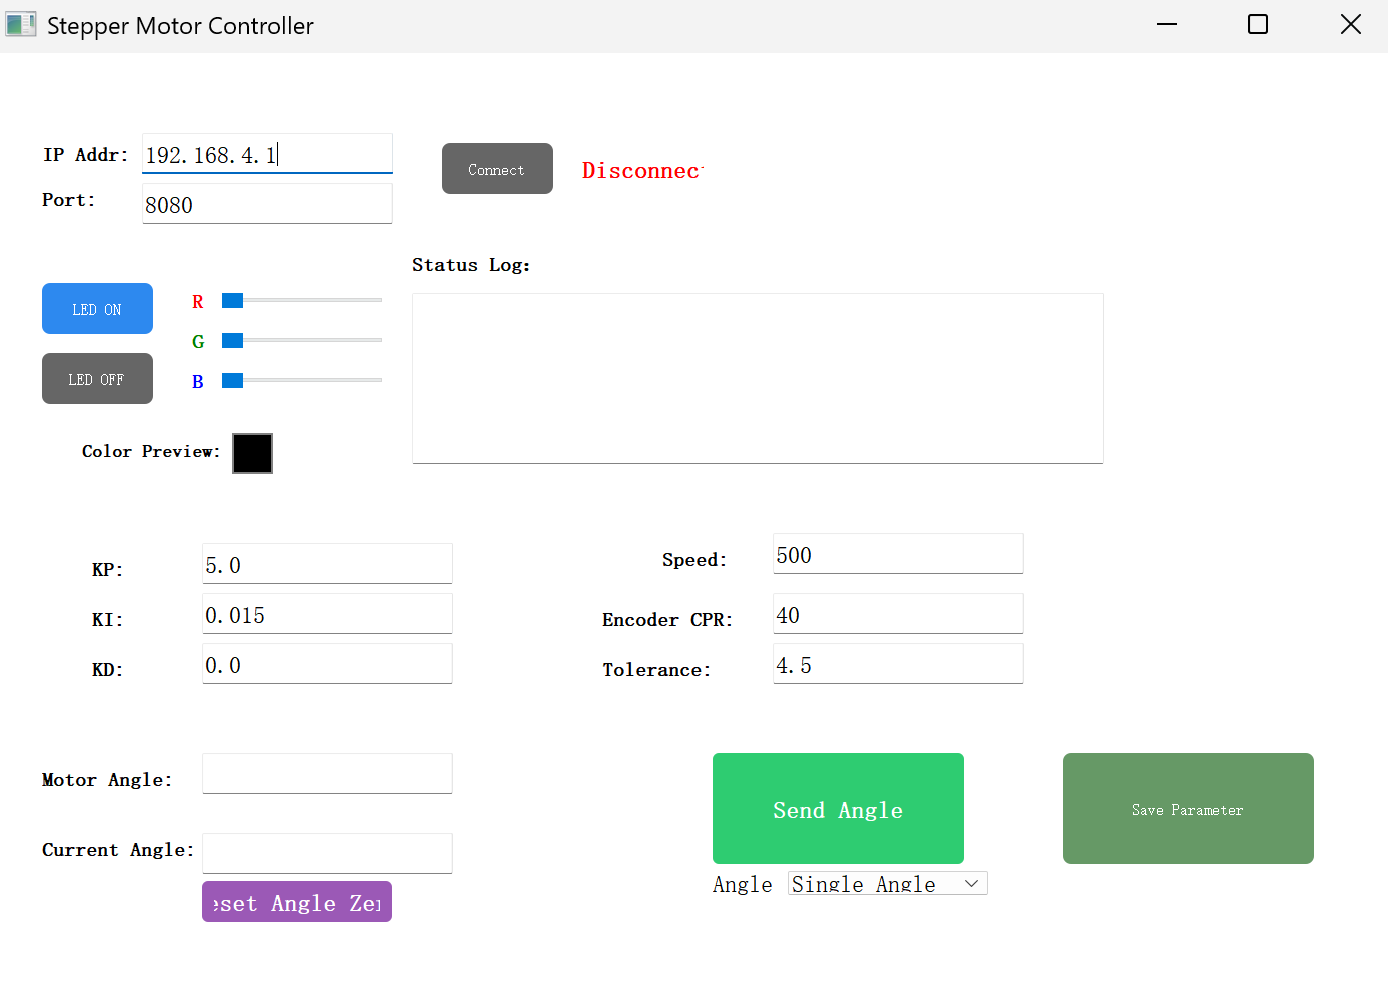
\includegraphics[width=0.6\textwidth]{qt_gui.png}
    \caption{Verbesserte Qt-Benutzeroberfläche zur Motorsteuerung}
    \label{fig:qt_gui}
\end{figure}

Insgesamt wurden sechs einstellbare Parameter in die Benutzeroberfläche integriert:

\begin{table}[H]
\centering
\caption{Einstellbare Parameter in der Benutzeroberfläche}
\renewcommand{\arraystretch}{1.2}
\begin{tabular}{ll}
\toprule
Parameter & Funktion \\
\midrule
\(K_p\) & Proportionalanteil des PID-Reglers \\
\(K_i\) & Integralanteil des PID-Reglers \\
\(K_d\) & Differentialanteil des PID-Reglers \\
Speed & Schrittfrequenz des Motors \\
Encoder CPR & Anzahl der Encoder-Impulse pro Umdrehung \\
Tolerance & Zulässige Abweichung zwischen Soll- und Istwinkel \\
\bottomrule
\end{tabular}
\end{table}

Nach dem Ändern der Parameter können diese über die Schaltfläche \textit{Save Parameter} an den ESP32-S3 gesendet werden. Anschließend werden die Werte im Flash-Speicher gespeichert. Dadurch bleiben die Einstellungen auch nach einem Neustart erhalten.

Das folgende Programmfragment zeigt die Übertragung der Parameter an den ESP32-S3:

\begin{verbatim}
sendCommand(QString("PID:%1,%2,%3").arg(kp).arg(ki).arg(kd));
sendCommand(QString("SPEED:%1").arg(speed));
sendCommand(QString("ENCODER:%1").arg(cpr));
sendCommand(QString("TOL:%1").arg(tol));

sendCommand("CFG_SAVE");
\end{verbatim}

Zusätzlich wurde eine Reset-Funktion ergänzt. Über die Schaltfläche \textit{Reset Angle Zero} kann die aktuell gespeicherte Winkelposition zurückgesetzt werden. Dabei wird der Befehl \texttt{ZERO} an den ESP32-S3 gesendet. Dadurch wird die aktuelle Position als neuer Nullpunkt verwendet und der gespeicherte Positionswert im Flash zurückgesetzt.

\begin{verbatim}
sendCommand("ZERO");
\end{verbatim}

Außerdem wurde die Motorsteuerung um verschiedene Betriebsarten erweitert. Im Modus \textit{Single Angle} wird ein einzelner Winkelbefehl an den ESP32-S3 gesendet. Nach Abschluss der Bewegung wartet die Benutzeroberfläche auf die Rückmeldung \texttt{MOTOR\_DONE}, bevor ein neuer Winkel gesendet werden kann.

Im Modus \textit{Back-and-Forth} wird der eingegebene Winkel abwechselnd in positiver und negativer Richtung gesendet. Dadurch kann der Motor automatisch eine wiederholte Hin- und Herbewegung ausführen. Diese Funktion ist besonders hilfreich, um das Regelverhalten, die Positioniergenauigkeit und die Stabilität des Systems über mehrere Bewegungszyklen zu testen.

Das folgende Programmfragment zeigt das Grundprinzip der Umschaltung zwischen Einzelbewegung und Hin- und Herbewegung:

\begin{verbatim}
if (currentAngleSendMode() == MODE_BACK_AND_FORTH) {
    gAngleSequenceRunning = true;
    gBackAndForthBaseAngle = angleValue;
    gBackAndForthSentCount = 1;
} else {
    gAngleSequenceRunning = false;
}

QString cmd = QString("ANGLE:%1").arg(formatAngleForCommand(firstAngle));
sendCommand(cmd);
\end{verbatim}

Die verbesserte Benutzeroberfläche erleichtert damit die Inbetriebnahme und Optimierung des Systems. Besonders die Fernparametrierung, das Speichern der Parameter im Flash, die Nullpunkt-Rücksetzung sowie die automatische Hin- und Herbewegung sind hilfreich, um das Verhalten des Motors unter verschiedenen Einstellungen zu untersuchen.



\end{document}
